\chapter{Survey}

\label{Chapter2}

\lhead{Chapter 2. \emph{Survey}}

\section{Similar problem domains} % (fold)
\label{survey:sec:similar_problem_domains}

Although the case in question is a specific service, the techniques in use and the limitations needing to be dealt with should apply to many kinds of applications.

Firstly, let's pick apart the workings of appear.in, to thoroughly understand what kind of an application we are dealing with -- a prerequisite for understanding the generated data and the applicability of the results herein for the general case.

\subsection{The inner workings of appear.in}
\label{survey:sub:appearin}

As illustrated in figure~\ref{fig:appearin-arch}, the appear.in architecture is quite simple. It is built on a simple peer-to-peer (P2P) architecture, with signaling done through a centralized server endpoint.

\begin{figure}[h]
  \centering
    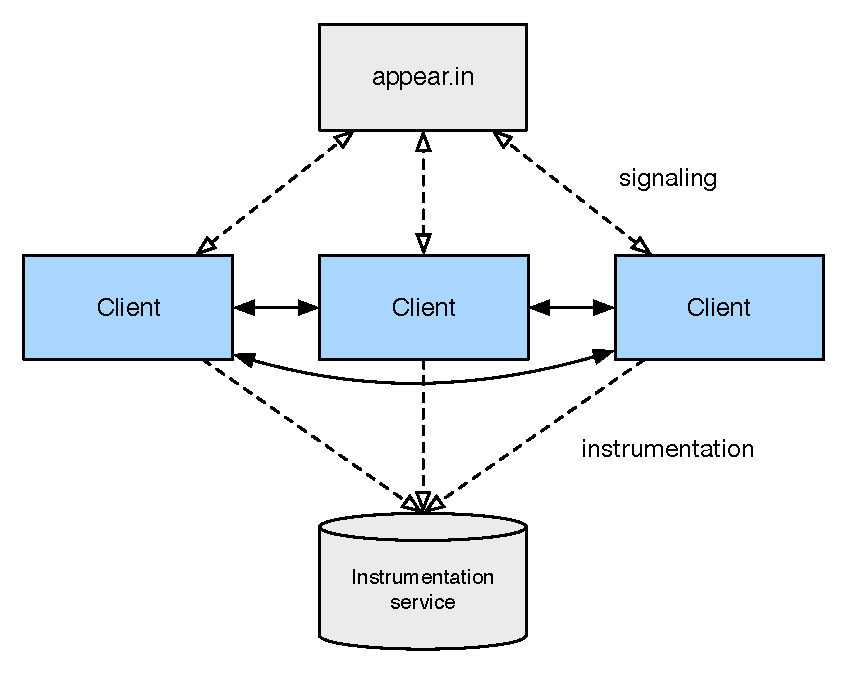
\includegraphics[width=0.9\textwidth]{Figures/appearin-arch}
    \caption{The appear.in architecture, illustrated for a conversation between 3 peers. \\ The black arrows indicate media data flow, and the dashed arrows indicate signaling data and instrumentation, as indicated.}
    \label{fig:appearin-arch}
\end{figure}

The instrumentation service has been included, simply to illustrate the fact that the data we have available is generated and sent directly from the clients.

By ``signaling'' in the context of appear.in, we mean everything not directly related to the media streams between the peers. This includes:

\begin{itemize}
  \item Managing which peers are in which room.
  \item Setting up new peer connections when a client joins a room.
  \item Tearing down peer connections when a client exits a room.
  \item Distributing various metadata that needs to be in sync across peers.
\end{itemize}

The user interface is also quite simple. It consists of a landing page (a screenshot of the current version can be seen in figure~\ref{fig:appearin-landing}), and a ``room page'' (see figure~\ref{fig:appearin-room}). For the sake of simplicity, let's go through them separately.

\subsubsection{The landing page}

\begin{figure}[h]
  \centering
    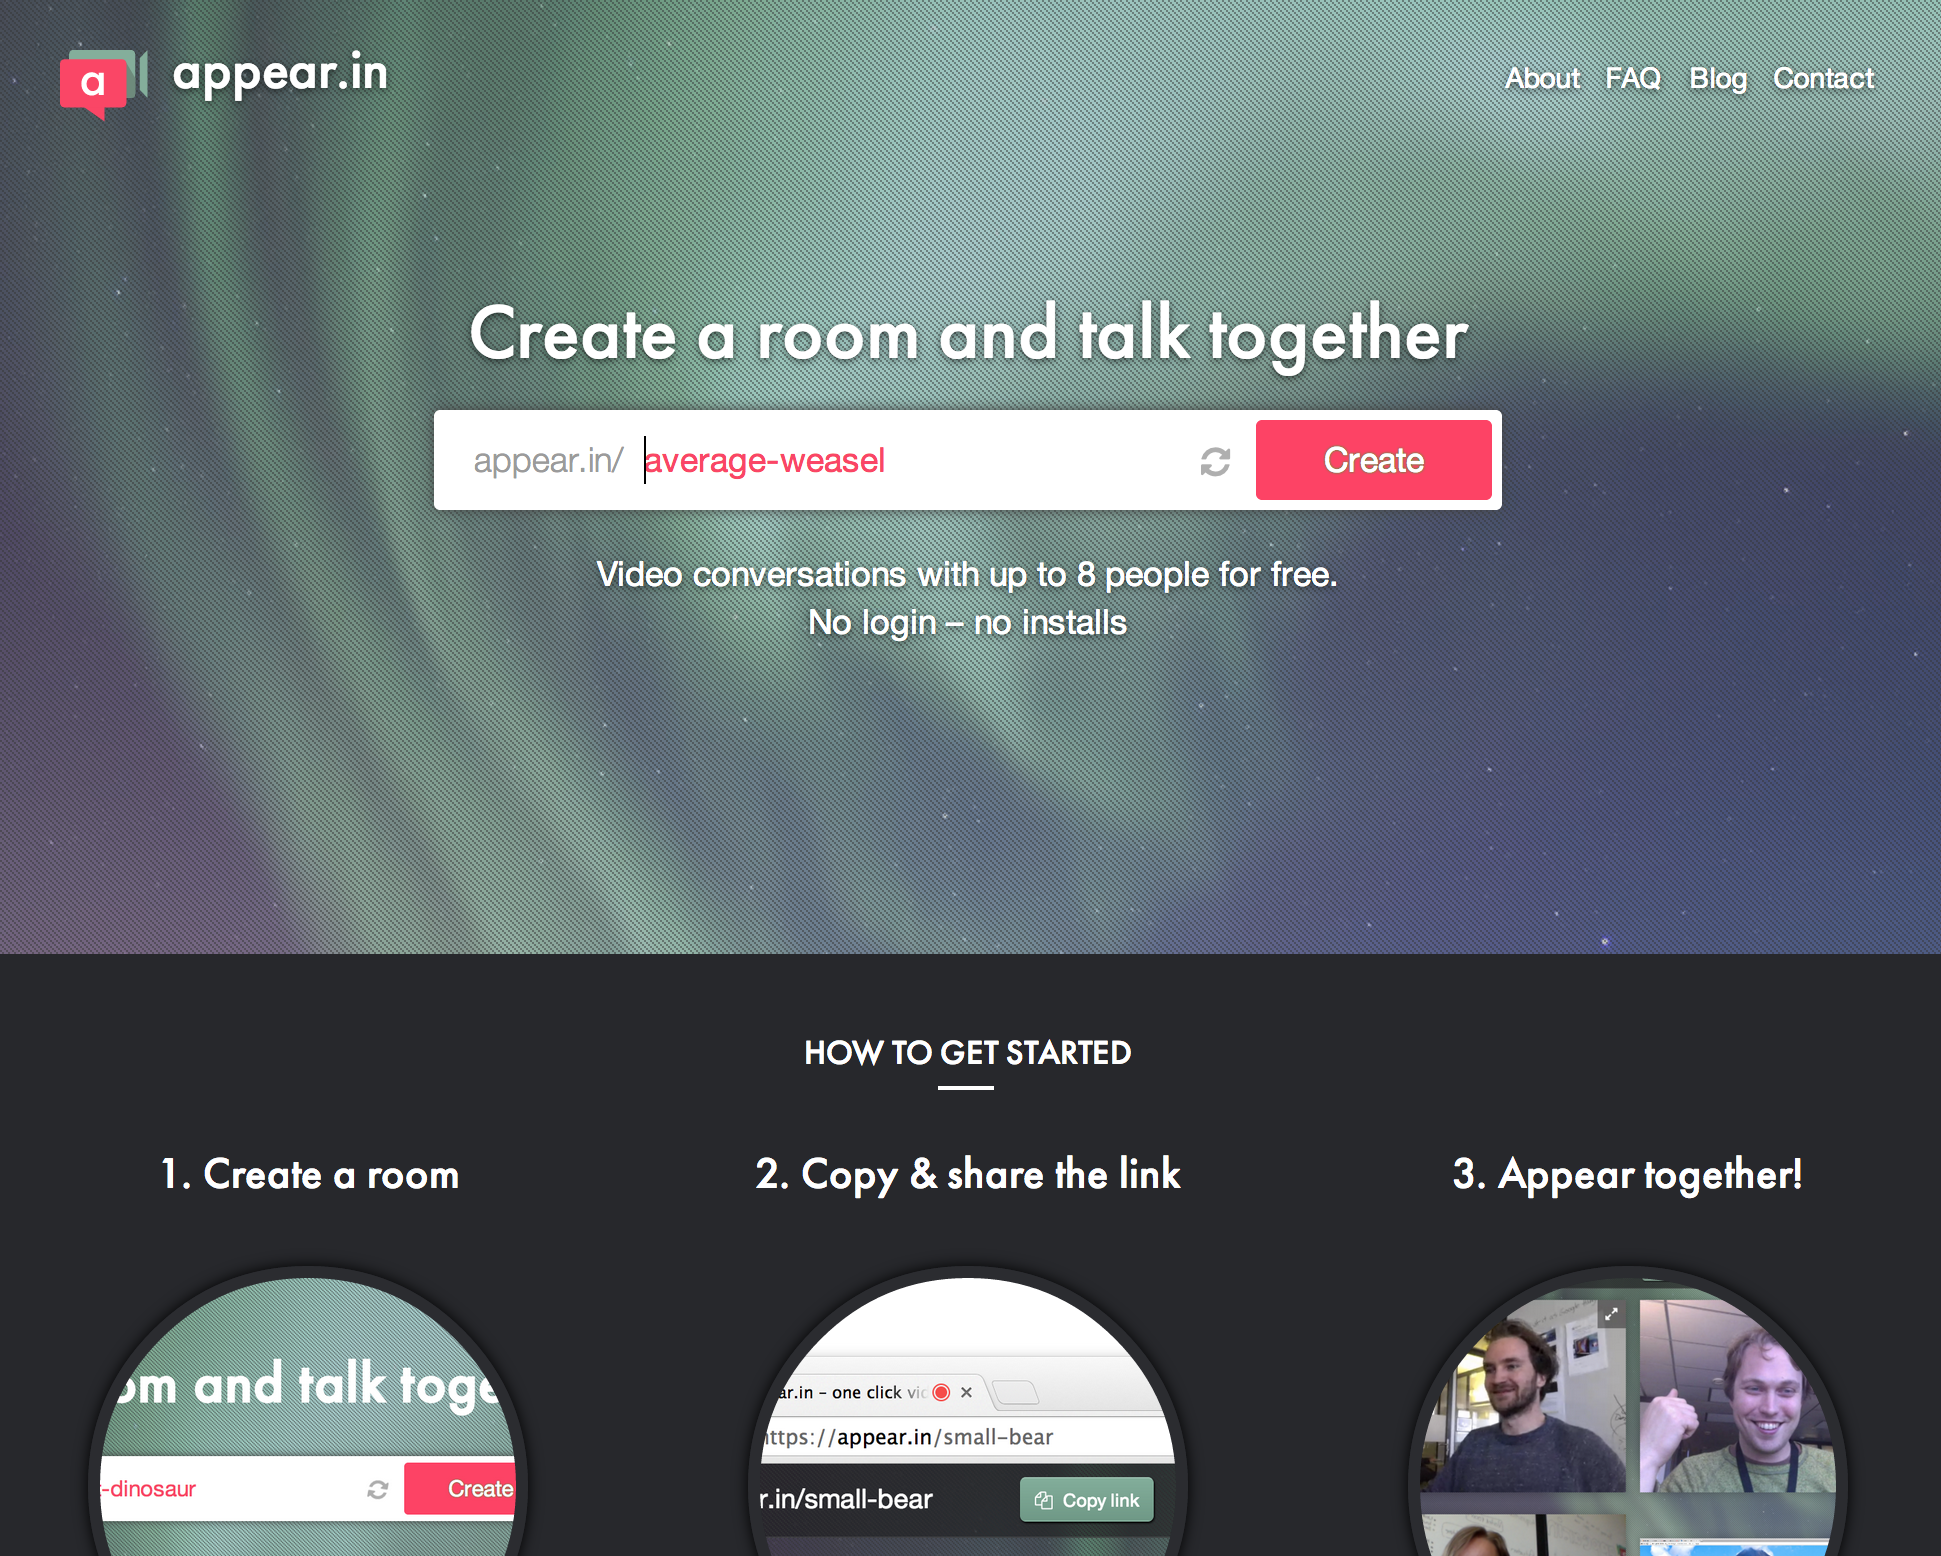
\includegraphics[width=\textwidth]{Figures/screenshots/appearin/frontpage-v2}
    \caption{The appear.in landing page (as of \today).}
    \label{fig:appearin-landing}
\end{figure}

The landing page's objective, as for most landing pages, is two-fold: to \emph{evoke interest}, and to \emph{activate the user}. Although we cannot directly measure them, we can indirectly measure the degree of interest and the activation rate in two ways:

\begin{enumerate}
  \item The ratio of users going from the landing page to a room (interest).
  \item The ratio of users going from the landing page to a room to a conversation (activation).
\end{enumerate}

The concept of evoking interest and of activating the user are universal terms that should generalize well to other web applications.

\subsubsection{The room page}

\begin{figure}[t]
  \centering
    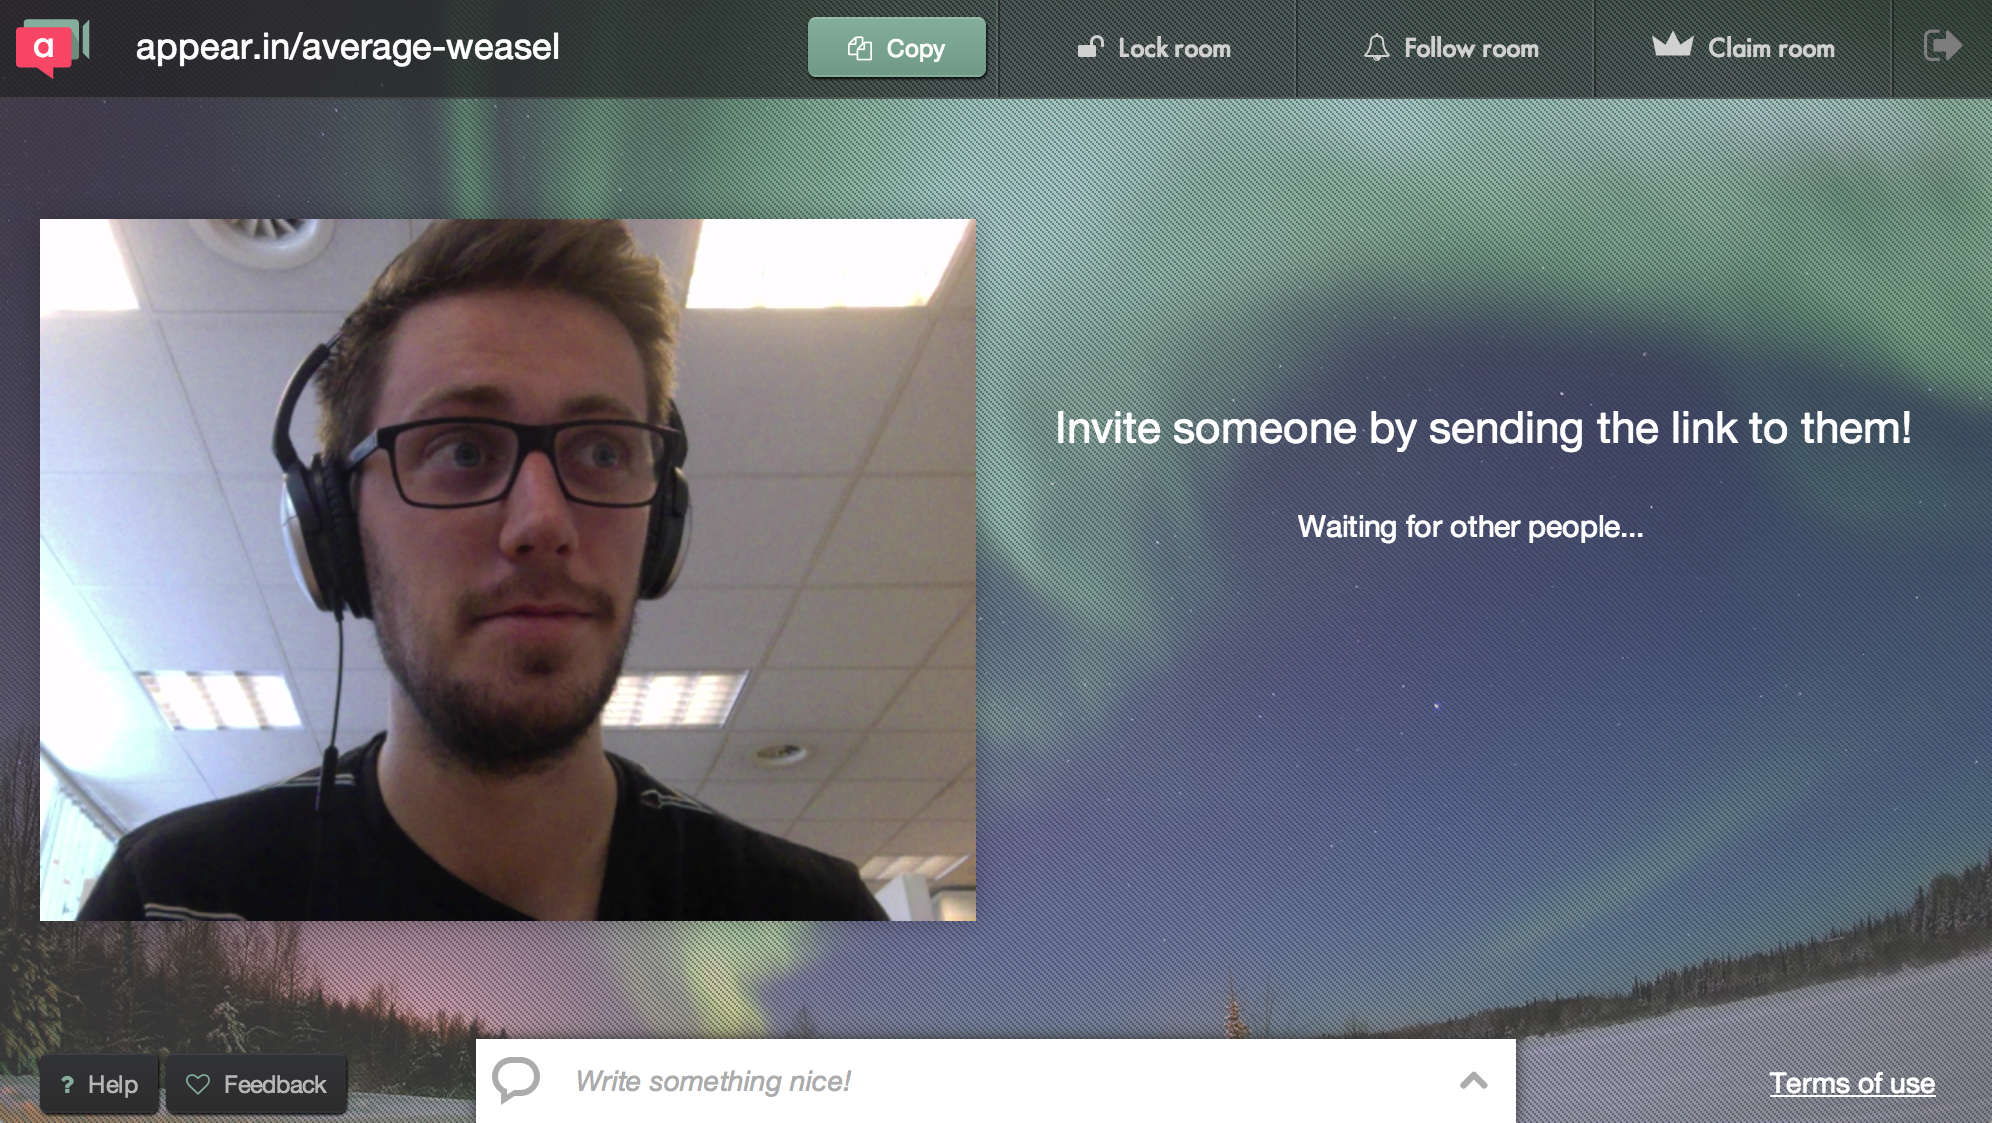
\includegraphics[width=\textwidth]{Figures/screenshots/appearin/in-room}
    \caption{The author in an appear.in room (as of \today).}
    \label{fig:appearin-room}
\end{figure}

The room page, the actual product user interface, is composed of several parts. Each participant resides in his or her own ``window'', and various room controls are placed along the top and bottom parts of the page.

As the quality of the video conferencing part of the application is largely governed by the browser and other low-level technicalities, we will mostly focus our efforts on the functionality augmenting the content: effectively, the rest of the UI.

\emph{Please note that all features discussed in this section are continuously subject to heavy revision, and should not in any way be viewed as a permanent or final set of features.}

The leftmost part of the top bar consists of a URL copying control, as shown in figure~\ref{fig:ui:copy_control}. Many users utilize this area when copying the page URL to invite their peers to the room. However, seeing as the same effect is easily achieved by copying the address field of the browser -- which we cannot track -- use of this control does not give a complete picture of users' sharing behavior.

To the top right is a row of buttons, as shown in figure~\ref{fig:ui:top_buttons}. Respectively, they allow the user to ``lock'', ``follow'', ``claim'', and leave the room. Of these, only the first three are of particular interest, as the ``leave room'' button essentially does nothing but close the window -- which we, again, cannot track.

All these buttons alter the state of the room. Let's briefly walk through them.

\begin{description}
  \item[Lock] \hfill \\
    When locking a room, one prevents other people stumbling upon the room's URL from entering. They are, however, able to knock their way in, much in the same fashion as one would enter a locked room in the physical world.
  \item[Follow] \hfill \\
    Users following a room are notified when other people enter it.
  \item[Claim] \hfill \\
    Users can claim a previously unclaimed room, and essentially take ownership of it. This enables them to customize the room in a number of ways.
\end{description}

The last piece of the feature puzzle is the chat control, depicted in figure~\ref{fig:ui:chat}. When users post a message, it becomes visible to other members. Chat messages are written to a centralized store, and persist as long as there are people in the room.

\begin{figure}[b]
  \centering
  \begin{subfigure}[t]{0.8\textwidth}
    
\includegraphics[width=\textwidth]{Figures/screenshots/appearin/feature-copy}
    \caption{The room URL copying control.}
    \label{fig:ui:copy_control}
  \end{subfigure}

  \vspace{.5cm}

  \begin{subfigure}[t]{0.95\textwidth}
    
\includegraphics[width=\textwidth]{Figures/screenshots/appearin/feature-chat}
    \caption{The chat control.}
    \label{fig:ui:chat}
  \end{subfigure}

  \vspace{.5cm}

  \begin{subfigure}[t]{0.95\textwidth}
    
\includegraphics[width=\textwidth]{Figures/screenshots/appearin/feature-buttons-top}
    \caption{The top button row. Each button serves its own purpose and fires its own event.}
    \label{fig:ui:top_buttons}
  \end{subfigure}

  \caption{The most important UI parts.}
  \label{fig:important_ui_parts}
\end{figure}

\subsection{Generality of the application case}
\label{survey:sub:generality}

To summarize section~\ref{survey:sub:appearin}, we will focus on the application features augmenting the main video conferencing functionality. These functions essentially either \emph{manipulate the room resource} or aid in \emph{exporting information} about it. Thus, the analyzed feature set should apply equally well to other applications where these are the central user tasks.

However, as touched upon in section~\ref{}, the main challenge with appear.in as an adaptation use-case is 1) the absence of demographics, and 2) the unreliability of user identity.

\subsubsection{The absence of demographics}

@TODO: refer to work involving demographics (surveys, webshops, marketing foobar etc.), work not requiring it (clickstream analysis, implicit user modeling etc), and work just talking about the issue.

The absence of demographics leaves us with less information for us to found our predictions on.

\subsubsection{The unreliability of user identity}
\label{survey:unreliable_identity}

Being an anonymous service, appear.in has no explicit login. As explained in section~\ref{intro:sub:tracking_users}, appear.in uses cookies to track users over time, which introduces some challenges when it comes to building user models.

Users periodically tend to clear browser cookies, which causes an abrupt end of the perceived event stream from the browser user, never to be reassumed. The effect is illustrated in figure~\ref{fig:clear_cookie_impact} for a hypothetical case, in which user $A$ clears the browser cache twice, effectively cutting off the event stream each time. There is no obvious way in which to consolidate the three event streams of the three perceived users $A$, $B$, and $C$.

\begin{figure}[h]
  \centering
    \begin{subfigure}[t]{0.8\textwidth}
      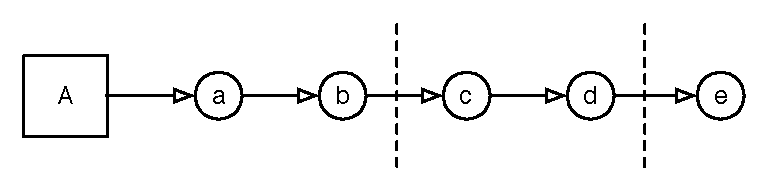
\includegraphics[width=\textwidth]{Figures/event-flow-cache-break-1}
      \caption{An event flow from $a \rightarrow e$, as seen from a user $A$. The dashed vertical lines indicate a point at which the user clears the browser cache.}
      \label{fig:cache_break1}
    \end{subfigure}
    \begin{subfigure}[t]{0.8\textwidth}
      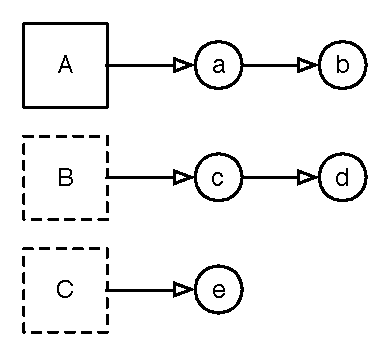
\includegraphics[width=0.5\textwidth]{Figures/event-flow-cache-break-2}
      \caption{The same event flow as perceived by the system.}
      \label{fig:cache_break2}
    \end{subfigure}

    \caption{The impact that clearing the browser cookies has on the chronological event stream for a single user $A$.}
    \label{fig:clear_cookie_impact}
\end{figure}

In practice, this leads to sparse usage data and quite a bit of noise in the event stream used as the foundation for the user model generation.

However, the shortening of event streams also introduces a bias to the clustering algorithms, as the user model vectors will be shorter than is actually the case. We will return to this issue in section~\ref{approach:sec:clustering}.

These are all issues that apply especially to appear.in, but that may also apply to many other anonymous systems.

\section{The field of user adaptation}
\label{survey:sec:user_adaptation}

This section will present an overview of the field of user adaptation. From the rather short history of the field, we move on to the conceptual frameworks and methodologies that modern adaptive systems base themselves on, before surveying the state of the art applications.

\subsection{A brief history of adaptive systems}
\label{survey:sec:adaptive_systems_history}

Vrieze discerns the history of adaptive systems into three eras~\cite{Vrieze}: early research, the pre-Internet era, and the Internet era. His historical dissertation is loosely based on Kobsa~\cite{Kobsa2001}. This summary will do the same, but focus on what Vrieze calls \emph{the Internet era}.

\subsubsection{Early research}

The first work within user modeling research was conducted in the nineteen-eighties. Strongly influenced by the field of artificial intelligence, the groundwork for modern user modeling was laid.

The common denominator for the user modeling systems composed in this era was their tight integration with their respective production systems. The end of the era, however, saw systems such as GUMS~\cite{Finin1989}, the first standalone user modeling system. These early standalone systems are most widely known as User Modeling Shell Systems, a term coined by Kobsa in 1990~\cite{Kobsa1990}.

\subsubsection{Pre-Internet research}

The nineteen-nineties was a decade widely dominated by User Modeling Shell Systems. Mostly, stereotype-based approaches were used, which sought to deduce logical connections between user models and the application domain.

One system, however, Doppelgänger~\cite{Orwant1995}, stands out in this regard, being the only system to employ a probabilistic model, and not a logic-based approach~\cite{Kobsa2001,Pohl1997,Pohl1999}.

\subsubsection{Internet-time research}

@TODO What are recent developments and key enablers?

\subsection{Personalization on the web}
\label{survey:sub:web_personalization}

When the field of user adaptation meets the web, we have traditionally tended to dub it either ``web personalization'' or ``adaptive hypermedia''. The terms are defined as follows:

\begin{description}
    \item[Web personalization] \hfill \\
      Any action that adapts the information or services provided by a Web site to the needs of a particular user or a set of users, taking advantage of the knowledge gained from the users' navigational behavior and individual interests, in combination with the content and the structure of the Web site~\cite{Eirinaki2003}.
    \item[Adaptive hypermedia] \hfill \\
      A hypertext or hypermedia system, with a user model, able to adapt the hypermedia using the model~\cite{Brusilovsky1996}.
\end{description}

The first definition assumes the website to be a hierarchy of content, whereas the second definition strongly relates to the concept of hypertext and hypermedia. However, large parts of the modern web have indeed shifted towards the application domain, as discussed in section~\ref{intro:sub:the_modern_web}, where the traditional concept of a website being some kind of structured set of ``content pages'' is completely outdated. In this light, these definitions are both a bit dated.

Recent research, however, usually does not make these kinds of assumptions about the form or structure of the systems being adapted, and is mostly quite applicable for the case of modern web applications.

Thus, we will be using the terms ``user adaptation'' and ``personalization'' without relating it to the domain in which it is visible to the user, as this is quite irrelevant with a clear separation of the application and adaptational component. The evolution of this model through the 90s and into the modern internet era is elaborated on in the following sections.

\subsection{Implementation methodology}

As mentioned, there are many approaches to the task of user adaptation. Due to the constraints outlined in the previous chapters, we will be honing in on the approach termed ``web usage mining'', or sometimes ``clickstream analysis''.

Traditionally, this has entailed tracking the way users traverse a website hierarchy, looking for path patterns among them, and using this information to adapt the pages in various ways~\cite{Mobasher2000,Eirinaki2003,Montgomery2009}. While not entirely the same, this is mostly analogous to the type of adaptation problem we are solving, and the systems proposed in this earlier work solves many of the same problems that we will need to solve.

% The following belongs in history, if anywhere. Outdated figure.
%
% A general, high-level sketch of a typical adaptive system is outlined in figure~\ref{fig:general_adaptive_system}.
%
% \begin{figure}[h]
%   \centering
%     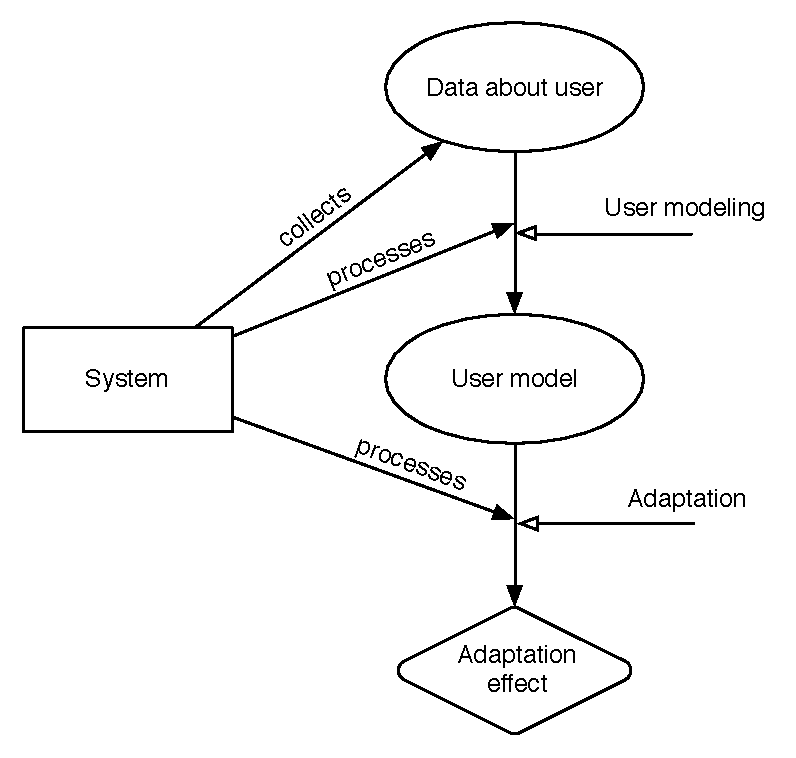
\includegraphics[width=0.8\textwidth]{Figures/adaptation-high-level}
%   \caption{Caption.}
%   \label{fig:general_adaptive_system}
% \end{figure}

\subsection{Privacy versus personalization}
\label{survey:sec:privacy_vs_personalization}

The marketing firm Jupiter defines personalization as ``predictive analysis of consumer data used to adapt targeted media, advertising and merchandising to consumer needs. According to Jupiter, personalization can be viewed as a cycle of recurring processes consisting of \emph{data collection}, \emph{profiling} and \emph{matching}''~\cite{Foster2000}. This section will discuss some ethical and political issues surrounding the first step of this cycle, namely \emph{data collection}.

Teltzrow and Kobsa~\cite{Teltzrow2004} state it plainly: ``Personalization systems need to acquire a certain amount of data about users' interests, behavior, demographics and actions before they can start adapting to them.'' As we shall see, many Internet users are highly sceptical of providing personal information to web sites, and a majority are concerned about web sites tracking their movements and behavior online. This doesn't fit adaptive systems' demand for data collection.

First, consider the following survey results regarding personal infomation~\cite{Teltzrow2004}:

\begin{enumerate}
  \item Internet Users who are concerned about the security of personal information: 83\% (Cyber Dialogue, 2001), 70\% (Behrens, 2001), 72\% (UMR, 2001), 84\% (Fox et al., 2000)
  \item People who have refused to give (personal) information to a web site: 82\% (Culnan and Milne, 2001)
  \item Internet users who would never provide personal information to a web site: 27\% (Fox et al., 2000)
  \item Internet users who supplied false or fictitious information to a web site when asked to register: 34\% (Culnan and Milne, 2001), 24\% (Fox et al., 2000)
\end{enumerate}

% @TODO: Resolve the above references into actual citations.

Although the above numbers aren't directly relevant to the case of appear.in, where no personal information is collected or stored, it underlines a general scepticism towards providing information to web sites.

The same scepticism is again seen when users are surveyed on their attitudes towards being tracked online~\cite{Teltzrow2004}.

\begin{enumerate}
  \item People who are concerned about being tracked on the Internet: 60\% (Cyber Dialogue, 2001), 54\% (Fox et al., 2000), 63\% (Harris, 2000)
  \item Internet users who generally accept cookies: 62\% (Personalization Consortium, 2000)
  \item Internet users who set their computers to reject cookies: 25\% (Culnan and Milne, 2001), 3\% (Cyber Dialogue, 2001), 31\% in warning modus (Cyber Dialogue, 2001), 10\% (Fox et al., 2000)
  \item Internet users who delete cookies periodically: 52\% (Personalization Consortium, 2000)
\end{enumerate}

Although these numbers are a bit dated, there is little reason to believe that the tracking situation is going to get any easier in the years to come. This is the subject of discussion in the next section.

As discussed in section~\ref{survey:unreliable_identity}, any time a user clears the browser cookies, we effectively break the user's event stream, and is from that moment onwards -- for all we know -- a brand new user.

This makes it hard to know if these numbers are similar to those among the users of appear.in, as they have not yet been surveyed on this subject. Furthermore, our only data source touching the user base is based on the tracking cookies in question -- hence we are unable to examine to what extent the above survey applies to our case.

\subsubsection{The road ahead}

\begin{itemize}
  \item Broad scepticism towards the use of cookies to track users, even on first-party sites.
  \item Legislation restricting the extent to which first-party, and especially third-party sites, can use cookies to track users has already been put into place -- with more to come.
\end{itemize}

\cite{RuizMartinez2012,Nikiforakis2013,Sorensen2013,Eijk2011}.

\section{Clustering techniques}
\label{survey:sec:clustering_techniques}

There are many approaches to the task of clustering user models.

@TODO: Some text on hierarchical, flat, density, probabilistic, k-median etc, before presenting k-means as our choice due to: good match with both input and desired output, scales well (parallel optimization), by far most popular in commercial applications~\cite{Berkhin2006}.

\subsection{Clustering evaluation}
\label{survey:sub:clustering_evaluation}

In general, any clustering method should search for clusters whose members are close to each other and well separated. Berry and Linoff~\cite{Berry1996} formulate it in terms of ``compactness'' and ``separation''.

\begin{description}
  \item[Compactness] \hfill \\
    The members of each cluster should be as close to each other as possible.
  \item[Separation] \hfill \\
    The clusters themselves should be widely spaced.
\end{description}

For an algorithm such as $k$-means, which takes the $k$ as an input, the central question when it comes to cluster validity is for which value of $k$ the cluster compactness and separation are optimal.

The most efficient way of measuring cluster quality between several executions of a clustering method, where only its parameters -- like $k$ -- differ, is to utilize a so-called \emph{relative criteria}~\cite{Halkidi2001}.

One of the most widely used measures of clusters' relative criteria is the Davies-Bouldin index, which is the one used to differentiate between clusters in this project. It is defined as:

\begin{equation}
  \text{DB}_k = \frac{1}{k} \sum_{i=1}^k \max_{i \neq j} \left( \frac{s_i + s_j}{d(c_i, c_j)} \right)
\end{equation}

where $k$ is the number of clusters, $c_x$ is the centroid of cluster $x$, $s_x$ is the average distance of all elements in cluster $x$ to centroid $c_x$, and $d(c_i,c_j)$ is the distance between centroids $c_i$ and $c_j$.

\section{A/B testing}
\label{survey:sec:ab_testing}

Controlled experiments embody the best scientific design for establishing a causal relationship between changes and their influence on user-observable behavior~\cite{Kohavi2007,Kohavi2008}.

The simplest form of controlled experiment is often referred to as the A/B test. In A/B tests users are randomly exposed to one of two variants: control (A), or treatment (B). Based on data collected, an Overall Evaluation Criterion (OEC) is derived for each variant. Figure~\ref{fig:ab_flow} illustrates the A/B testing process.

@TODO: Insert figure similar to the one in Kohavi2007 p.3.

One word in the previous paragraph, ``randomly'', warrants some discussion. To be able to establish a causal relationship between the selected variant and the evaluation, the variant selection must indeed be completely random, and not based on what Kohavi et al. term ``any old which way''~\cite{Kohavi2007}.

This point \emph{must} be kept in mind when designing adaptive systems based on controlled experiments, as in our case.

\section{State of the art}
\label{survey:sub:state_of_the_art}



% \section{Similar research} % (fold)
% \label{survey:sec:similar_applications}
%
% The approach taken to adaptive personalization is based heavily on the work by Vrieze in ``Fundaments of Adaptive Personalization''~\cite{Vrieze}.
%
% \subsection{Relevant literature} % (fold)
% \label{survey:sec:relevant_literature}
%
% Teltzrow and Kobsa's work on privacy-driven personalization systems provides insight into a lot of the issues surrounding the lack of demographic information in personalization~\cite{Teltzrow2004,Kobsa2007}. However, the main focus of their work seems to be that users are more willing to provide demographic information if that information is not backtracable to themselves, through pseudonymous personalization.
% This matches the application in question quite poorly, as the goal is not to obtain demographics -- rather to attempt to cope without it.
%
% \emph{@TODO} Explore and include literature on:
%
% \begin{itemize}
%   \item Clustering and segmenting users, choice of algorithms etc.
%   \item Visualizing and evaluating clusters.
%   \item A/B testing, multivariate testing, multi-arm bandits.
%   \item Motivations for adaptive personalization. Online business models?
%   \item Anonymity: do users experience personalization as an overstep?
% \end{itemize}
